\section{Proposed Methodology}
\label{sec:method}

RA-PatchTST keeps the PatchTST backbone unchanged and adds three components (Fig.~\ref{fig:arch}). This section first describes data preparation and the backbone, then each addition, the corruption model used for training and testing, and the training objective.

\begin{figure*}[!t]
\centering
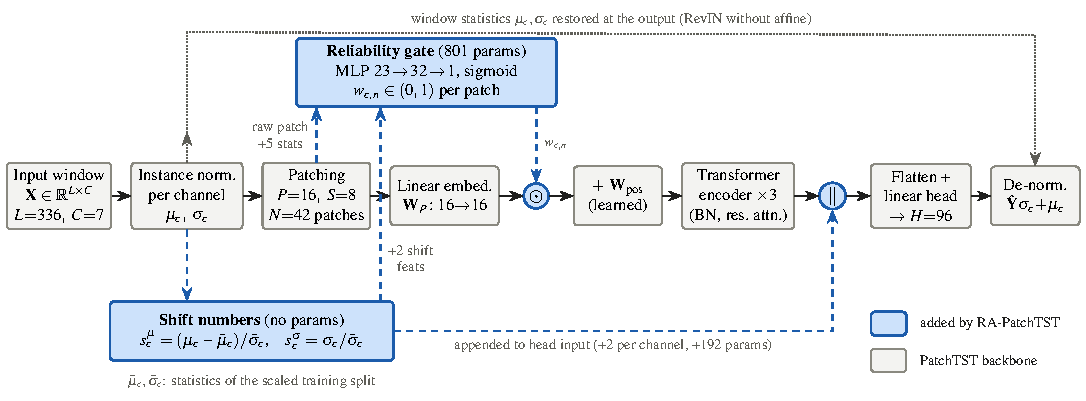
\includegraphics[width=\figwidth]{fig_architecture.pdf}
\caption{RA-PatchTST architecture. Grey blocks are the PatchTST backbone; blue blocks are the components added in this work. The reliability gate scores every patch and rescales its embedding before the position encoding is added; the two shift numbers are computed from the window statistics that instance normalization removes and are appended to the input of the linear head. Corruption-aware training (Fig.~\ref{fig:cat}) changes only the data fed to this network.}
\label{fig:arch}
\end{figure*}

\subsection{Data Preparation}
\label{sec:method-data}

The series is split chronologically into training, validation and test segments (Section~\ref{sec:exp}). A per-channel z-score scaler is fitted on the training segment only and applied to all three,
\begin{equation}
\begin{gathered}
\bar{s}_{t,c}=\frac{s_{t,c}-m_c}{d_c},\qquad m_c=\frac{1}{T_{\mathrm{tr}}}\sum_{t\le T_{\mathrm{tr}}}s_{t,c},\\
d_c^2=\frac{1}{T_{\mathrm{tr}}}\sum_{t\le T_{\mathrm{tr}}}(s_{t,c}-m_c)^2,
\end{gathered}
\label{eq:scale}
\end{equation}
so that no validation or test statistics leak into training. Windows of length $L+H$ are then cut with stride 1. Validation and test windows start $L$ steps before their segment so that the first forecast target lies exactly on the segment border, as in the Time-Series-Library protocol~\cite{tslib_code}. We also store the per-channel mean $\bar{\mu}_c$ and standard deviation $\bar{\sigma}_c$ of the \emph{scaled} training segment, which the shift features use. By construction $\bar{\mu}_c=0$ and $\bar{\sigma}_c=1$ up to rounding; the code keeps them explicit so that the same model can be used with other scalers.

\subsection{PatchTST Backbone}
\label{sec:method-backbone}

\subsubsection{Instance normalization}
For each window and channel the model computes
\begin{equation}
\begin{gathered}
\mu_c=\frac{1}{L}\sum_{i=1}^{L}x_{i,c},\qquad \sigma_c=\sqrt{\frac{1}{L}\sum_{i=1}^{L}(x_{i,c}-\mu_c)^2+\varepsilon},\\
x^{N}_{i,c}=\frac{x_{i,c}-\mu_c}{\sigma_c},
\end{gathered}
\label{eq:revin}
\end{equation}
with $\varepsilon=10^{-5}$. The statistics are treated as constants during back-propagation. This is RevIN~\cite{revin} without the learnable affine parameters, matching the configuration of the official PatchTST script for ETTh1.

\subsubsection{Patching}
Each normalized channel $\mathbf{x}^{N}_{c}\in\R^{L}$ is padded at the end with $S$ copies of its last value and unfolded into overlapping patches of length $P$ with stride $S$ (Fig.~\ref{fig:patching}):
\begin{equation}
\begin{gathered}
\mathbf{p}_{c,n}=\big[x^{N}_{nS+1,c},\dots,x^{N}_{nS+P,c}\big]^{\top}\in\R^{P},\\
n=0,\dots,N-1,\qquad N=\Big\lfloor\frac{L-P}{S}\Big\rfloor+2.
\end{gathered}
\label{eq:patch}
\end{equation}
With $L=336$, $P=16$ and $S=8$ this gives $N=42$ patches per channel, hence the name PatchTST/42.

\begin{figure}[!t]
\centering
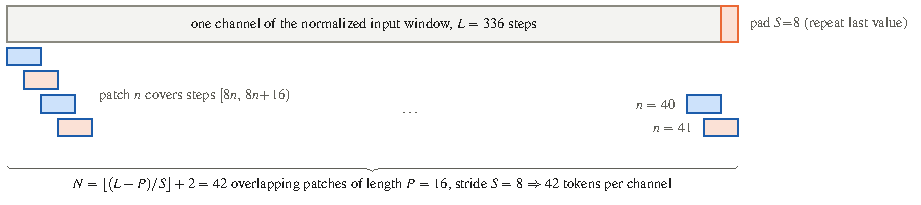
\includegraphics[width=\colfig]{fig_patching.pdf}
\caption{Patching of one channel. End padding with $S$ repeated values adds one patch, giving $N=42$ tokens for $L=336$, $P=16$, $S=8$.}
\label{fig:patching}
\end{figure}

\subsubsection{Embedding and encoder}
Each patch is mapped to a $D$-dimensional token by a shared linear layer, and a learnable position encoding $\mathbf{W}_{\mathrm{pos}}\in\R^{N\times D}$ is added:
\begin{equation}
\mathbf{e}_{c,n}=\mathbf{W}_P\,\mathbf{p}_{c,n}+\mathbf{b}_P,\qquad \mathbf{u}^{(0)}_{c,n}=\mathbf{e}_{c,n}+\mathbf{W}_{\mathrm{pos},n}.
\label{eq:embed}
\end{equation}
Channels are processed independently: the batch of $B$ windows becomes $B\cdot C$ sequences of $N$ tokens. Each of the three encoder layers applies multi-head self-attention with residual attention scores~\cite{realformer}, followed by a position-wise feed-forward network, each wrapped in a residual connection and BatchNorm~\cite{batchnorm}. For head $h$ in layer $l$,
\begin{equation}
\begin{gathered}
\mathbf{A}^{(l)}_h=\frac{\mathbf{Q}^{(l)}_h{\mathbf{K}^{(l)}_h}^{\top}}{\sqrt{d_k}}+\mathbf{A}^{(l-1)}_h,\\
\mathrm{head}^{(l)}_h=\mathrm{softmax}\big(\mathbf{A}^{(l)}_h\big)\,\mathbf{V}^{(l)}_h,
\end{gathered}
\label{eq:attn}
\end{equation}
where $\mathbf{A}^{(0)}_h=\mathbf{0}$ and $d_k=D/n_h$. The layer output is
\begin{align}
\mathbf{z}^{(l)}&=\mathrm{BN}\big(\mathbf{u}^{(l-1)}+\mathrm{Drop}(\mathrm{MHA}(\mathbf{u}^{(l-1)})\mathbf{W}_O)\big),\label{eq:layer1}\\
\mathbf{u}^{(l)}&=\mathrm{BN}\big(\mathbf{z}^{(l)}+\mathrm{Drop}(\mathbf{W}_2\,\mathrm{GELU}(\mathbf{W}_1\mathbf{z}^{(l)}))\big),\label{eq:layer2}
\end{align}
with GELU activation~\cite{gelu} and dropout~\cite{dropout}. We use $D=16$, $n_h=4$, a feed-forward width of 128 and dropout 0.3, the official settings for ETTh1.

\subsubsection{Head and de-normalization}
The $N$ output tokens of each channel are flattened into $\mathbf{h}_c\in\R^{ND}$ ($ND=672$), mapped to the horizon by a linear head, and the window statistics are restored:
\begin{equation}
\hat{\mathbf{y}}^{N}_c=\mathbf{W}_H\mathbf{h}_c+\mathbf{b}_H\in\R^{H},\qquad \hat{\mathbf{y}}_c=\sigma_c\,\hat{\mathbf{y}}^{N}_c+\mu_c.
\label{eq:head}
\end{equation}

\subsection{Patch Reliability Gate}
\label{sec:method-gate}

The gate is a small MLP that assigns every patch a weight $w_{c,n}\in(0,1)$ (Fig.~\ref{fig:gate}). Its input concatenates the 16 normalized values of the patch with seven summary features:
\begin{equation}
\begin{split}
\mathbf{g}_{c,n}=\mathrm{clip}_{[-10,10]}\Big(\big[&\mathbf{p}_{c,n};\ \bar{p}_{c,n};\ \varsigma_{c,n};\ j_{c,n};\\
&z_{c,n};\ a_{c,n};\ s^{\mu}_c;\ s^{\sigma}_c\big]\Big)\in\R^{23}.
\end{split}
\label{eq:gatein}
\end{equation}
Here $\bar{p}_{c,n}$ and $\varsigma_{c,n}$ are the mean and standard deviation of the patch, and $a_{c,n}=\max_k|p_{c,n,k}|$ is its largest absolute value. The jump feature compares a patch's mean with the average of its neighbours,
\begin{equation}
j_{c,n}=\Big|\bar{p}_{c,n}-\tfrac12\big(\bar{p}_{c,n-1}+\bar{p}_{c,n+1}\big)\Big|,
\label{eq:jump}
\end{equation}
with the first and last patch mean repeated at the borders. The zero share $z_{c,n}$ is the fraction of values in the corresponding patch of the \emph{un-normalized} (scaled) input that are exactly zero; it was designed to expose missing values, which the corruption model fills with the training mean, i.e., zero after scaling. The last two entries are the window-level shift features defined in~\eqref{eq:shift} below, broadcast to every patch of the channel. The gate is
\begin{equation}
w_{c,n}=\mathrm{sigmoid}\Big(\mathbf{v}_2^{\top}\,\mathrm{ReLU}\big(\mathbf{V}_1\mathbf{g}_{c,n}+\mathbf{c}_1\big)+c_2\Big),
\label{eq:gate}
\end{equation}
with $\mathbf{V}_1\in\R^{32\times23}$, $\mathbf{c}_1,\mathbf{v}_2\in\R^{32}$ and $c_2\in\R$. The weight rescales the patch embedding before the position encoding is added, replacing~\eqref{eq:embed} by
\begin{equation}
\mathbf{u}^{(0)}_{c,n}=w_{c,n}\big(\mathbf{W}_P\,\mathbf{p}_{c,n}+\mathbf{b}_P\big)+\mathbf{W}_{\mathrm{pos},n}.
\label{eq:gated}
\end{equation}
Applying the gate before the position encoding means that a fully distrusted patch still occupies its position in the sequence but carries no content. The output bias is initialized to $c_2=4$, so that $w\approx\mathrm{sigmoid}(4)\approx0.982$ at the start of training and the model initially behaves like PatchTST. The gate has $23\cdot32+32+32+1=801$ parameters. No supervision tells the gate which patches are corrupted; it is trained only through the forecasting loss. The code also supports an optional penalty $\lambda(1-\bar{w})$ that discourages uniformly low weights, but it was not used ($\lambda=0$) in any reported run.

\begin{figure}[!t]
\centering
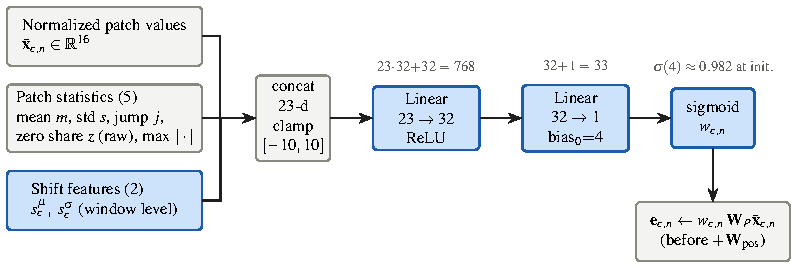
\includegraphics[width=\linewidth]{fig_gate.pdf}
\caption{Reliability gate. Each patch is scored from its 16 normalized values, five patch statistics and the two shift features of its channel. The score multiplies the patch embedding.}
\label{fig:gate}
\end{figure}

\subsection{Shift-Aware Head}
\label{sec:method-shift}

Instance normalization~\eqref{eq:revin} makes the encoder blind to where a window sits relative to the data the model was trained on: a window whose level has moved by two standard deviations looks the same after normalization as an ordinary one. The window statistics are added back at the output~\eqref{eq:head}, but only as an affine correction, so the shape of the forecast cannot depend on them. We compute two shift numbers per channel,
\begin{equation}
s^{\mu}_c=\frac{\mu_c-\bar{\mu}_c}{\bar{\sigma}_c},\qquad s^{\sigma}_c=\frac{\sigma_c}{\bar{\sigma}_c},
\label{eq:shift}
\end{equation}
and append them to the flattened encoder output before the head:
\begin{equation}
\hat{\mathbf{y}}^{N}_c=\mathbf{W}'_H\big[\mathbf{h}_c;\ s^{\mu}_c;\ s^{\sigma}_c\big]+\mathbf{b}_H,\qquad \mathbf{W}'_H\in\R^{H\times(ND+2)}.
\label{eq:shifthead}
\end{equation}
This adds $2H=192$ parameters. The idea is related to the de-stationary attention of Non-stationary Transformers~\cite{nstransformer}, which also reinjects removed statistics, but here they enter only the linear head. The same two numbers feed the gate.

\subsection{Corruption Model}
\label{sec:method-corrupt}

All corruptions act on scaled input windows, so a unit of one corresponds to one training standard deviation. Let $\mathbf{M}$ denote the mask of altered positions, $\odot$ the element-wise product and $\mathcal{B}(p)$ an independent Bernoulli draw per position.

\textit{Missing values (point):} $\mathbf{M}\sim\mathcal{B}(p)$ and $\tilde{\X}=(\mathbf{1}-\mathbf{M})\odot\X$, i.e., each dropped value is replaced by the training mean (zero).

\textit{Missing values (16-step stretch):} a stretch starts at each position with probability $p/16$ and zeroes the next 16 values of that channel, so the expected coverage is close to $p$ and a whole patch length can be lost at once.

\textit{Noise:} $\mathbf{M}\sim\mathcal{B}(p)$ and $\tilde{\X}=\X+\mathbf{M}\odot\bm{\epsilon}$ with $\epsilon_{i,c}\sim\mathcal{N}(0,1)$.

\textit{Anomaly (spike):} $\mathbf{M}\sim\mathcal{B}(p)$ and $\tilde{\X}=\X+\mathbf{M}\odot\mathbf{r}\odot\mathbf{a}$ with magnitudes $a_{i,c}\sim\mathcal{U}(3,5)$ and random signs $r_{i,c}\in\{-1,+1\}$.

\textit{Shift:} for each window and channel, $k$ segments of length $\lfloor L/10\rfloor=33$ with random start are transformed as
\begin{equation}
\tilde{x}_{i,c}=\alpha\,x_{i,c}+\beta,\qquad \alpha\sim\mathcal{U}(0.5,2),\quad \beta\sim\mathcal{U}(-2,2),
\label{eq:shiftcorr}
\end{equation}
with independent $(\alpha,\beta)$ per segment. Segments may overlap.

\textit{Mixed:} shift with $k=1$, then noise, spikes and point-wise missing values, each at $p=5\%$. Missing values are applied last so that dropped values stay exactly zero.

The severity levels are $p\in\{1,5,10,15\}\%$ of points for the first four types and $k\in\{1,3,5,10\}$ segments for shift. Fig.~\ref{fig:corr} shows each type on a real test window.

\begin{figure*}[!t]
\centering
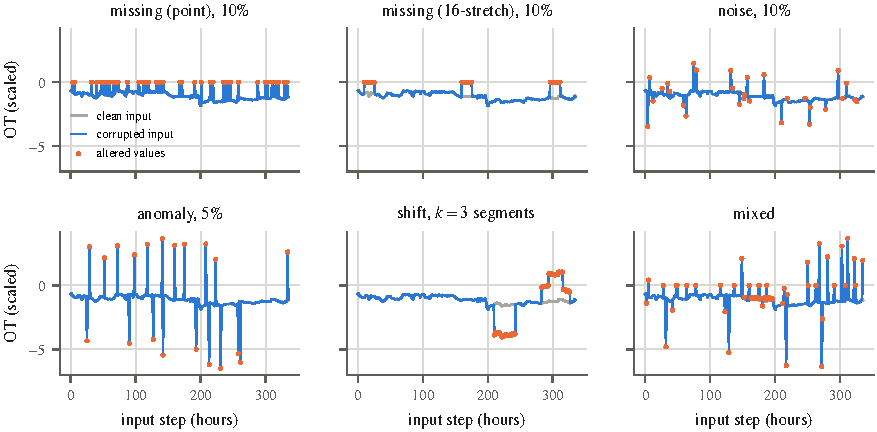
\includegraphics[width=\figwidth]{fig_corruptions.pdf}
\caption{The corruption types applied to one ETTh1 test input window (oil temperature channel, scaled units). Grey: clean input; blue: corrupted input; orange dots: altered values. The panels were drawn with a NumPy port of the project's corruption functions using the same distributions and parameters.}
\label{fig:corr}
\end{figure*}

\subsection{Corruption-Aware Training}
\label{sec:method-cat}

During training each window in a mini-batch is corrupted independently with probability $0.5$ (Fig.~\ref{fig:cat}). For a corrupted window the type is drawn uniformly from \{missing, noise, anomaly, shift\} and the level index uniformly from the four levels; a missing-value corruption is point-wise or stretch-wise with equal probability. The mixed setting is never used for training. The loss~\eqref{eq:mse} is always computed against the clean future, so the network learns to forecast the true continuation from damaged evidence. Because corruption is drawn afresh at every step, the model sees a different damaged copy of each window in every epoch.

\begin{figure}[!t]
\centering
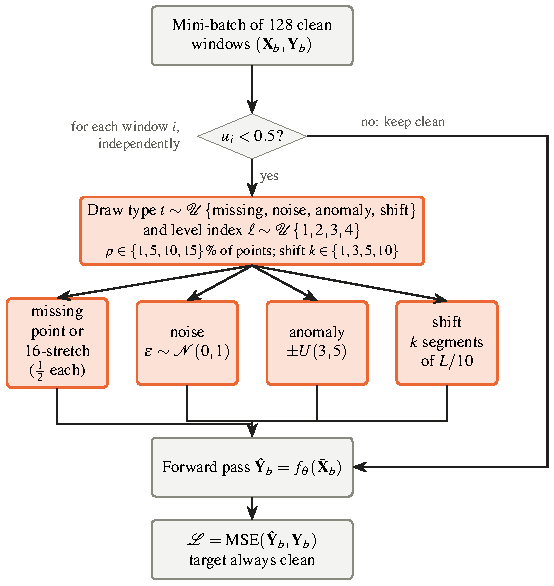
\includegraphics[width=\colfig]{fig_cat.pdf}
\caption{Corruption-aware training. Each window of a mini-batch is corrupted with probability 0.5 using a randomly chosen type and severity. The forecasting loss always uses the clean target.}
\label{fig:cat}
\end{figure}

\subsection{Optimization and Model Selection}
\label{sec:method-opt}

All variants use Adam~\cite{adam} with an initial learning rate $\eta_0=10^{-4}$, batch size 128 and the step decay of the official code (its ``type3'' schedule),
\begin{equation}
\eta_e=\eta_0\cdot0.9^{\max(0,\,e-4)},\qquad e=1,2,\dots
\label{eq:lr}
\end{equation}
Training runs for at most 20 epochs. After each epoch we evaluate the validation MSE on clean windows and on a fixed mixed-corruption copy of the validation set, and keep the checkpoint that minimizes
\begin{equation}
J=\tfrac12\big(\mathrm{MSE}_{\mathrm{val}}^{\mathrm{clean}}+\mathrm{MSE}_{\mathrm{val}}^{\mathrm{mixed}}\big).
\label{eq:select}
\end{equation}
Early stopping uses the same criterion with patience 5. We also keep the checkpoint with the lowest clean validation MSE, which is used only to report the clean reproduction of PatchTST. Algorithm~\ref{alg:train} summarizes the procedure.

\begin{algorithm}[!t]
\caption{Training and selection of one RA-PatchTST variant}
\label{alg:train}
\small
\begin{algorithmic}[1]
\Require training windows $\mathcal{D}_{\mathrm{tr}}$, validation windows $\mathcal{D}_{\mathrm{va}}$, variant flags (gate, shift head, CAT), seed
\State $\tilde{\mathcal{D}}_{\mathrm{va}}\gets$ mixed corruption of $\mathcal{D}_{\mathrm{va}}$ with seed 777
\State initialize $\theta$; gate output bias $c_2\gets4$; $J^\star\gets\infty$; $bad\gets0$
\For{$e=1$ \textbf{to} $20$}
  \State $\eta\gets10^{-4}\cdot0.9^{\max(0,e-4)}$
  \For{each mini-batch $(\X_b,\Y_b)$ of 128 windows, shuffled, last partial batch dropped}
    \If{CAT} \State $\X_b\gets$ corrupt each window with probability 0.5 (random type and level) \EndIf
    \State $\hat{\Y}_b\gets f_\theta(\X_b)$ \Comment{Eqs.~\eqref{eq:revin}--\eqref{eq:shifthead}}
    \State $\theta\gets\mathrm{Adam}\big(\theta,\nabla_\theta\,\mathrm{MSE}(\hat{\Y}_b,\Y_b),\eta\big)$
  \EndFor
  \State $J\gets\frac12\big(\mathrm{MSE}(f_\theta,\mathcal{D}_{\mathrm{va}})+\mathrm{MSE}(f_\theta,\tilde{\mathcal{D}}_{\mathrm{va}})\big)$
  \If{$J<J^\star$} \State $J^\star\gets J$;\ $\theta^\star\gets\theta$;\ $bad\gets0$ \Else \State $bad\gets bad+1$ \EndIf
  \If{$bad\ge5$} \textbf{break} \EndIf
\EndFor
\State \Return $\theta^\star$
\end{algorithmic}
\end{algorithm}

\subsection{Model Variants}
\label{sec:method-variants}

The ablation adds one component at a time (Table~\ref{tab:variants}). A0 is the PatchTST baseline. A1 adds corruption-aware training only, so it isolates the effect of the training data. A2 and A3 add the shift-aware head and the gate respectively on top of A1, and A4 is the full RA-PatchTST. Two further variants are defined in the code, A5 (A4 without corruption-aware training) and A6 (A4 with a gate that does not see the shift features), but they were not run and no result is reported for them.

\begin{table}[!t]
\centering
\caption{Model Variants of the Ablation}
\label{tab:variants}
\footnotesize
\colfit{%
\begin{tabular}{@{}lcccrl@{}}
\toprule
Variant & CAT & Shift head & Gate & Params & Status \\
\midrule
A0 PatchTST & -- & -- & -- & 81,728 & run, 2 seeds \\
A1 & \checkmark & -- & -- & 81,728 & run, 2 seeds \\
A2 & \checkmark & \checkmark & -- & 81,920 & run, 2 seeds \\
A3 & \checkmark & -- & \checkmark & 82,529 & run, 2 seeds \\
A4 RA-PatchTST & \checkmark & \checkmark & \checkmark & 82,721 & run, 2 seeds \\
A5 & -- & \checkmark & \checkmark & 82,721 & defined, not run \\
A6 & \checkmark & \checkmark & \checkmark$^{\dagger}$ & 82,657 & defined, not run \\
\bottomrule
\multicolumn{6}{@{}p{0.95\linewidth}@{}}{\scriptsize CAT: corruption-aware training. $^{\dagger}$Gate without the two shift features (21 inputs instead of 23).}
\end{tabular}}
\end{table}

\subsection{Complexity}
\label{sec:method-complexity}

For a batch of $B$ windows, self-attention costs $O(B\,C\,N^2 D)$ per layer and the feed-forward network $O(B\,C\,N\,D\,d_{ff})$. The gate adds $O(B\,C\,N\cdot(23\cdot32+32))$ operations, roughly the cost of one extra feed-forward layer of width 32 on the patch tokens, and the shift head adds $O(B\,C\,H)$. Neither changes the asymptotic cost. The parameter count of the backbone breaks down as follows: patch embedding 272, position encoding 672, three encoder layers of 5,392 each (attention projections 1,088, two BatchNorms 64, feed-forward 4,240) and the head 64,608, for 81,728 in total. The head dominates, and the gate and shift head together add 993 parameters (1.2\%).
